\documentclass[12pt, a4paper, twoside, titlepage]{article}
\usepackage[utf8]{inputenc}
\usepackage[english]{babel}
\usepackage{amsmath}
\usepackage{amsfonts}
\usepackage{amssymb}
\usepackage{gensymb}
\usepackage{graphicx}
\usepackage[dvipsnames]{xcolor}
\usepackage{tikz}
\usetikzlibrary{arrows,automata,shapes}
\tikzstyle{decision} = [diamond, draw, fill=blue!20, text width=4.5em, text badly centered, node distance=2.5cm, inner sep=0pt]
\tikzstyle{block} = [rectangle, draw, fill=blue!20, text width=5em, text centered, rounded corners, minimum height=4em]
\tikzstyle{line} = [draw, very thick, color=black!50, -latex']
\tikzstyle{cloud} = [draw, ellipse,fill=red!20, node distance=2.5cm,minimum height=2em]

\definecolor{LightGray}{gray}{0.9}
\definecolor{NormalGray}{gray}{0.8}
\definecolor{DarkGray}{gray}{0.7}

\title{Libre Silicon process specification}
\date{\today} 
\author{David Lanzendörfer}

\begin{document}
\maketitle

\begin{abstract}
	Copyright © 2017 LANCEVILLE TECHNOLOGY GROUP CO., LIMITED. All rights reserved. \\

	This process is licensed under the Libre Silicon public license; you can redistribute it and/or modify it under the terms of the Libre Silicon public license
	as published by the Libre Silicon alliance, either version 2 of the License, or (at your option) any later version.

	This design is distributed in the hope that it will be useful, but WITHOUT ANY WARRANTY; without even the implied warranty of MERCHANTABILITY or FITNESS FOR A PARTICULAR PURPOSE.
	See the Libre Silicon Public License for more details. \\

	This is the specification of the free silicon manufacturing standard for manufacturing the ls018\footnotemark standard logic cells and related free technology nodes from the LibreSilicon project.
	\footnotetext[1]{https://github.com/leviathanch/ls018}
\end{abstract}

\section{Overall process}
Below the general flow chart of the overall process flow can be seen. These process steps will be discussed within the following sections.
\begin{center}
	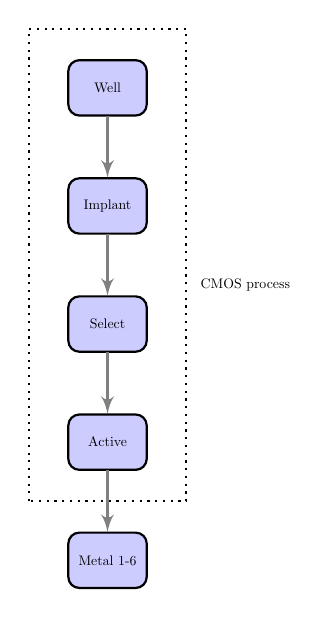
\begin{tikzpicture}[node distance = 3cm, auto, thick,scale=0.5, every node/.style={transform shape}]
		% Place nodes
		\node [block] (well) {Well};
		\node [block, below of=well] (implant) {Implant};
		\node [block, below of=implant] (select) {Select};
		\node [block, below of=select] (active) {Active};
		\node [block, below of=active] (metal) {Metal 1-6};
		% Draw edges
		\path [line] (well) -- (implant);
		\path [line] (implant) -- (select);
		\path [line] (select) -- (active);
		\path [line] (active) -- (metal);
		
		\draw[dotted] (-2,-10.5) rectangle (2,1.5);
		\node at (3.5,-5) {CMOS process};
	\end{tikzpicture}
\end{center}
The four starting overall process steps are part of an overall active part of the technology, while the final metal (respectively contact) layers will be used for making a contact between the logic gates and macro cells and making them available to the exterior world.
For this process p-substrate is the required basic substrate, but forks and modifications will be very well possible based on a Graphene substrate or alike, still under the LSPL.

\section{Well}
\subsection{Dioxide layer}
\begin{center}
	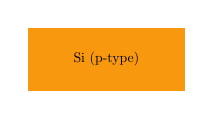
\begin{tikzpicture}[node distance = 3cm, auto, thick,scale=0.5, every node/.style={transform shape}]
		% substrate
		\fill[YellowOrange] (0,0) rectangle (4,1.6);
		\node at (2,0.8) {Si (p-type)};
	\end{tikzpicture}
	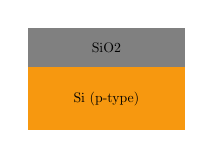
\begin{tikzpicture}[node distance = 3cm, auto, thick,scale=0.5, every node/.style={transform shape}]
		% substrate
		\fill[YellowOrange] (0,0) rectangle (4,1.6);
		\node at (2,0.8) {Si (p-type)};
		% oxide
		\fill[gray] (0,1.6) rectangle (4,2.6);
		\node at (2,2.1) {SiO2};
	\end{tikzpicture}
\end{center}
In order to selectively inject charge carrying atoms into the crystalline structure a protective dioxide ($SiO_2$) layer needs to be grown on top of a p-type substrate.
There is no clear general equation perfectly describing the absorption behavior of silicon dioxide but the industrial best practice is a layer of around 1$\mu$m (1000nm) thickness.

\subsection{Pattering and etching}
\begin{center}
	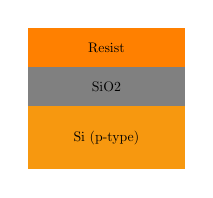
\begin{tikzpicture}[node distance = 3cm, auto, thick,scale=0.5, every node/.style={transform shape}]
		% substrate
		\fill[YellowOrange] (0,0) rectangle (4,1.6);
		\node at (2,0.8) {Si (p-type)};
		% oxide
		\fill[gray] (0,1.6) rectangle (4,2.6);
		\node at (2,2.1) {SiO2};
		% resist
		\fill[orange] (0,2.6) rectangle (4,3.6);
		\node at (2,3.1) {Resist};
	\end{tikzpicture}
	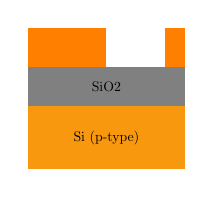
\begin{tikzpicture}[node distance = 3cm, auto, thick,scale=0.5, every node/.style={transform shape}]
		% substrate
		\fill[YellowOrange] (0,0) rectangle (4,1.6);
		\node at (2,0.8) {Si (p-type)};
		% oxide
		\fill[gray] (0,1.6) rectangle (4,2.6);
		\node at (2,2.1) {SiO2};
		% resist 1
		\fill[orange] (0,2.6) rectangle (2,3.6);
		% resist 2
		\fill[orange] (3.5,2.6) rectangle (4,3.6);
	\end{tikzpicture}
	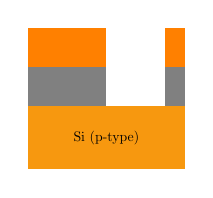
\begin{tikzpicture}[node distance = 3cm, auto, thick,scale=0.5, every node/.style={transform shape}]
		% substrate
		\fill[YellowOrange] (0,0) rectangle (4,1.6);
		\node at (2,0.8) {Si (p-type)};
		% oxide 1
		\fill[gray] (0,1.6) rectangle (2,2.6);
		% oxide 2
		\fill[gray] (3.5,1.6) rectangle (4,2.6);
		% resist 1
		\fill[orange] (0,2.6) rectangle (2,3.6);
		% resist 2
		\fill[orange] (3.5,2.6) rectangle (4,3.6);
	\end{tikzpicture}
\end{center}
The resist is being deposited using spin coating and then baked depending on the baking time for the specific resist.
The layout for being exposed onto the resist is being extracted from the "nwell" layer within the GDS2 file.

\subsection{Infusion}
\begin{center}
	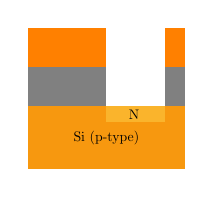
\begin{tikzpicture}[node distance = 3cm, auto, thick,scale=0.5, every node/.style={transform shape}]
		% substrate
		\fill[YellowOrange] (0,0) rectangle (4,1.6);
		\node at (2,0.8) {Si (p-type)};
		% oxide 1
		\fill[gray] (0,1.6) rectangle (2,2.6);
		% oxide 2
		\fill[gray] (3.5,1.6) rectangle (4,2.6);
		% resist 1
		\fill[orange] (0,2.6) rectangle (2,3.6);
		% resist 2
		\fill[orange] (3.5,2.6) rectangle (4,3.6);
		% well
		\fill[Dandelion] (2,1.2) rectangle (3.5,1.6);
		\node at (2.7,1.4) {N};
	\end{tikzpicture}
\end{center}
The decision to use an n-well approach is based largely on the compatibility with the existing nMOS process.
The starting material is a p-type, <100> oriented silicon with a doping concentration of $\approx 9\times10^{14}cm^{-3}$.
The n-well is implanted with a $P^{31}$ dose of $2.5\times10^{12}cm^{-2}$ at an energy of 100 KeV.
The n-well is then annealed, oxidized for 32 minutes at 1000\degree C, and then driven-in for 960 minutes at 1150\degree C in an inert ambient.

\section{Implant}
\section{Select}
\section{Active}
\begin{center}
	%\begin{tikzpicture}[node distance = 3cm, auto, thick,scale=0.5, every node/.style={transform shape}]
	\begin{tikzpicture}
		% substrate
		\fill[YellowOrange] (0,0) rectangle (4,1.6);
		\node at (2,0.8) {Si (p-type)};

		%% active regions 1:
		% p-active 1
		\fill[blue] (0,1.3) rectangle (0.5,1.6);
		% p-active 2
		\fill[blue] (1.55,1.3) rectangle (2.05,1.6);
		% p-active 3
		\fill[blue] (3.5,1.3) rectangle (4,1.6);

		% oxide 1
		\fill[NormalGray] (0,1.6) rectangle (0.5,2);
		% oxide 2
		\fill[NormalGray] (1.55,1.6) rectangle (2.05,2);
		% oxide 3
		\fill[NormalGray] (3.5,1.6) rectangle (4,2);

		%% active regions 2
		% gate oxide 1
		\fill[DarkGray] (0.9,1.6) rectangle (1.1,1.7);
		% gate oxide 2
		\fill[DarkGray] (2.45,1.6) rectangle (2.65,1.7);
		% poly 1
		\fill[red] (0.9,1.7) rectangle (1.1,2);
		% poly 2
		\fill[red] (2.45,1.7) rectangle (2.65,2);

		% n-active 1
		\fill[green] (0.55,1.4) rectangle (0.95,1.6);
		% n-active 2
		\fill[green] (1.05,1.4) rectangle (1.45,1.6);

		% n-well
		\fill[Dandelion] (2.1,1.2) rectangle (3.45,1.6);
		\node at (2.7,1.4) {N};
		
		% p-active nwell 1
		\fill[blue] (2.15,1.4) rectangle (2.5,1.6);
		% p-active nwell 2
		\fill[blue] (2.6,1.4) rectangle (2.95,1.6);
		% n-active nwell 1
		\fill[green] (3.1,1.4) rectangle (3.3,1.6);

	\end{tikzpicture}
\end{center}
\section{Metal}


\end{document}